% A0 portrait conference poster — Vitrine
% University of Salford AI Knowledge-Exchange CoP pilot · DreamLab AI Consulting Ltd
% Build (from report/poster/):  pdflatex poster_a0.tex
\documentclass[25pt, a0paper, portrait, margin=10mm, innermargin=12mm,
               blockverticalspace=10mm, colspace=13mm, subcolspace=8mm]{tikzposter}

\usepackage[utf8]{inputenc}
\usepackage[T1]{fontenc}
\usepackage[british]{babel}
\usepackage{helvet}
\renewcommand{\familydefault}{\sfdefault}
\usepackage{graphicx}
\usepackage{amsmath}
\usepackage{amssymb}
\usepackage{booktabs}
\usepackage{tabularx}
\usepackage{array}
\usepackage{xcolor}
\usepackage{colortbl}
\usepackage{tikz}
\usetikzlibrary{arrows.meta, positioning, shapes.geometric, calc, fit, backgrounds}

\graphicspath{{../figures/v2/}{../figures/v3/}{../figures/}{./assets/}}

% ---------------------------------------------------------------------------
% University of Salford brand palette (primary red + supporting tones).
% salfordred is the single point of truth — update here if the brand hex moves.
% ---------------------------------------------------------------------------
\definecolor{salfordred}{HTML}{D20A11}   % primary Salford red (official 2025 brand)
\definecolor{salforddeep}{HTML}{8E060B}  % deepened red for inner titles
\definecolor{salfordnavy}{HTML}{0F172A}  % near-black slate
\definecolor{salfordblack}{HTML}{1D1D1B}
\definecolor{salfordteal}{HTML}{6FB6BA}  % secondary cool accent (brand teal)
\definecolor{salfordgold}{HTML}{F6C900}  % warm accent (brand gold)
\definecolor{panelgrey}{HTML}{F4F1EC}    % warm panel background
\definecolor{linegrey}{HTML}{C9C3B8}
\definecolor{dreamlabnavy}{HTML}{0B1020}
\definecolor{dreamlabindigo}{HTML}{6366F1}
\definecolor{okgreen}{HTML}{15803D}

\usetheme{Default}
\usecolorstyle{Germany}
\colorlet{backgroundcolor}{white}
\colorlet{framecolor}{salfordred}
\colorlet{titlefgcolor}{salfordred}
\colorlet{titlebgcolor}{white}
\colorlet{blocktitlebgcolor}{salfordred}
\colorlet{blocktitlefgcolor}{white}
\colorlet{blockbodybgcolor}{white}
\colorlet{blockbodyfgcolor}{salfordblack}
\colorlet{innerblocktitlebgcolor}{salfordnavy}
\colorlet{innerblocktitlefgcolor}{white}
\colorlet{notebgcolor}{panelgrey}
\colorlet{notefrcolor}{salfordred}

\useblockstyle[titlewidthscale=1.0, bodywidthscale=1.0]{Default}
\usetitlestyle{Empty}

\setlength{\parindent}{0pt}
% Big red statistic with a unit suffix
\newcommand{\stat}[2]{{\color{salfordred}\bfseries #1}\,{\footnotesize #2}}
% Small status tag
\newcommand{\stag}[2]{\textcolor{#1}{\footnotesize\textbf{#2}}}

% ---------------------------------------------------------------------------
% Branded title band: Salford crest (prominent, left) · title · DreamLab (right)
% ---------------------------------------------------------------------------
\settitle{
\begin{minipage}[c]{0.255\linewidth}
  
\includegraphics[width=0.97\linewidth]{salford_logo.png}
\end{minipage}%
\hfill
\begin{minipage}[c]{0.60\linewidth}
  \centering
  {\color{salfordred}\bfseries\fontsize{96}{104}\selectfont Vitrine\,{\color{salfordgold}//}}\\[5mm]
  {\color{salfordnavy}\fontsize{37}{45}\selectfont Agentic Volumetric Capture for the Preservation of\\[1mm]
   Immersive \& Intangible Cultural Heritage}\\[7mm]
  {\color{salfordblack}\fontsize{25}{31}\selectfont One hand-held walkthrough video $\rightarrow$ a photoreal, \emph{object-resolved} 3D scene graph,\\[1mm]
   ready for a games engine}\\[7mm]
  {\color{salfordred}\bfseries\fontsize{23}{29}\selectfont University of Salford \quad{\color{salfordgold}/}\quad AI Knowledge-Exchange Community of Practice Pilot}\\[2mm]
  {\color{salfordnavy}\fontsize{21}{27}\selectfont delivered in partnership with DreamLab AI Consulting Ltd}
\end{minipage}%
\hfill
\begin{minipage}[c]{0.125\linewidth}
  \centering
  \colorbox{dreamlabnavy}{\makebox[0.97\linewidth][c]{\rule{0pt}{0pt}
\includegraphics[width=0.80\linewidth]{dreamlab_logo.png}}}
\end{minipage}
}

\begin{document}
\maketitle[width=0.98\textwidth]

% Thin full-width programme strap under the title (must be a tikzposter block,
% not a raw center env — body content lives on the poster's tikz canvas).
{\useblockstyle{Minimal}
\colorlet{blockbodybgcolor}{panelgrey}
\block{}{\centering\color{salfordnavy}\large
\textbf{Programme team:} Roger McKinley (Creative Technology \& Content Manager, lead)\;$\cdot$\;
Glenn Watts (Immersive Technology, MetaCampus)\;$\cdot$\;
Derek Hales (Academic Architect, advisory)\;$\cdot$\;
Dr John O'Hare (DreamLab AI, technical lead)\hspace{6mm}
{\color{salfordred}\textbf{Worktribe 5043317}}}}
\vspace{2mm}

\begin{columns}

% ======================================================================
% COLUMN 1
% ======================================================================
\column{0.34}

\block{Preservation Gap}{
The University of Salford holds a growing catalogue of immersive, experiential,
time-based arts (\textbf{Nested Cinema}, \textbf{We Invented the Weekend},
\textbf{Lightwaves}), yet has \textbf{no efficient pipeline to preserve or
re-stage} these site-based experiences once the event is over. Cultural heritage
of this kind is fragile, immovable and under-documented; flat photography and
sparse photogrammetry lose material appearance, view-dependent light and the
spatial relationships between objects.
\vspace{3mm}

This pilot tests a working route from \textbf{existing 2D assets} (a single
hand-held 4K video) to \textbf{3D objects that live inside a games engine}, the
Salford MetaCampus in Unreal. The aim, in the bid's own words: an
\emph{efficient, automated AI agentic workflow to transcribe video and 2D media
into 3D objects for the emulation and preservation of cultural assets}.
\vspace{4mm}

\begin{tikzfigure}[A single 4K walkthrough of a gallery interior is the only input.]
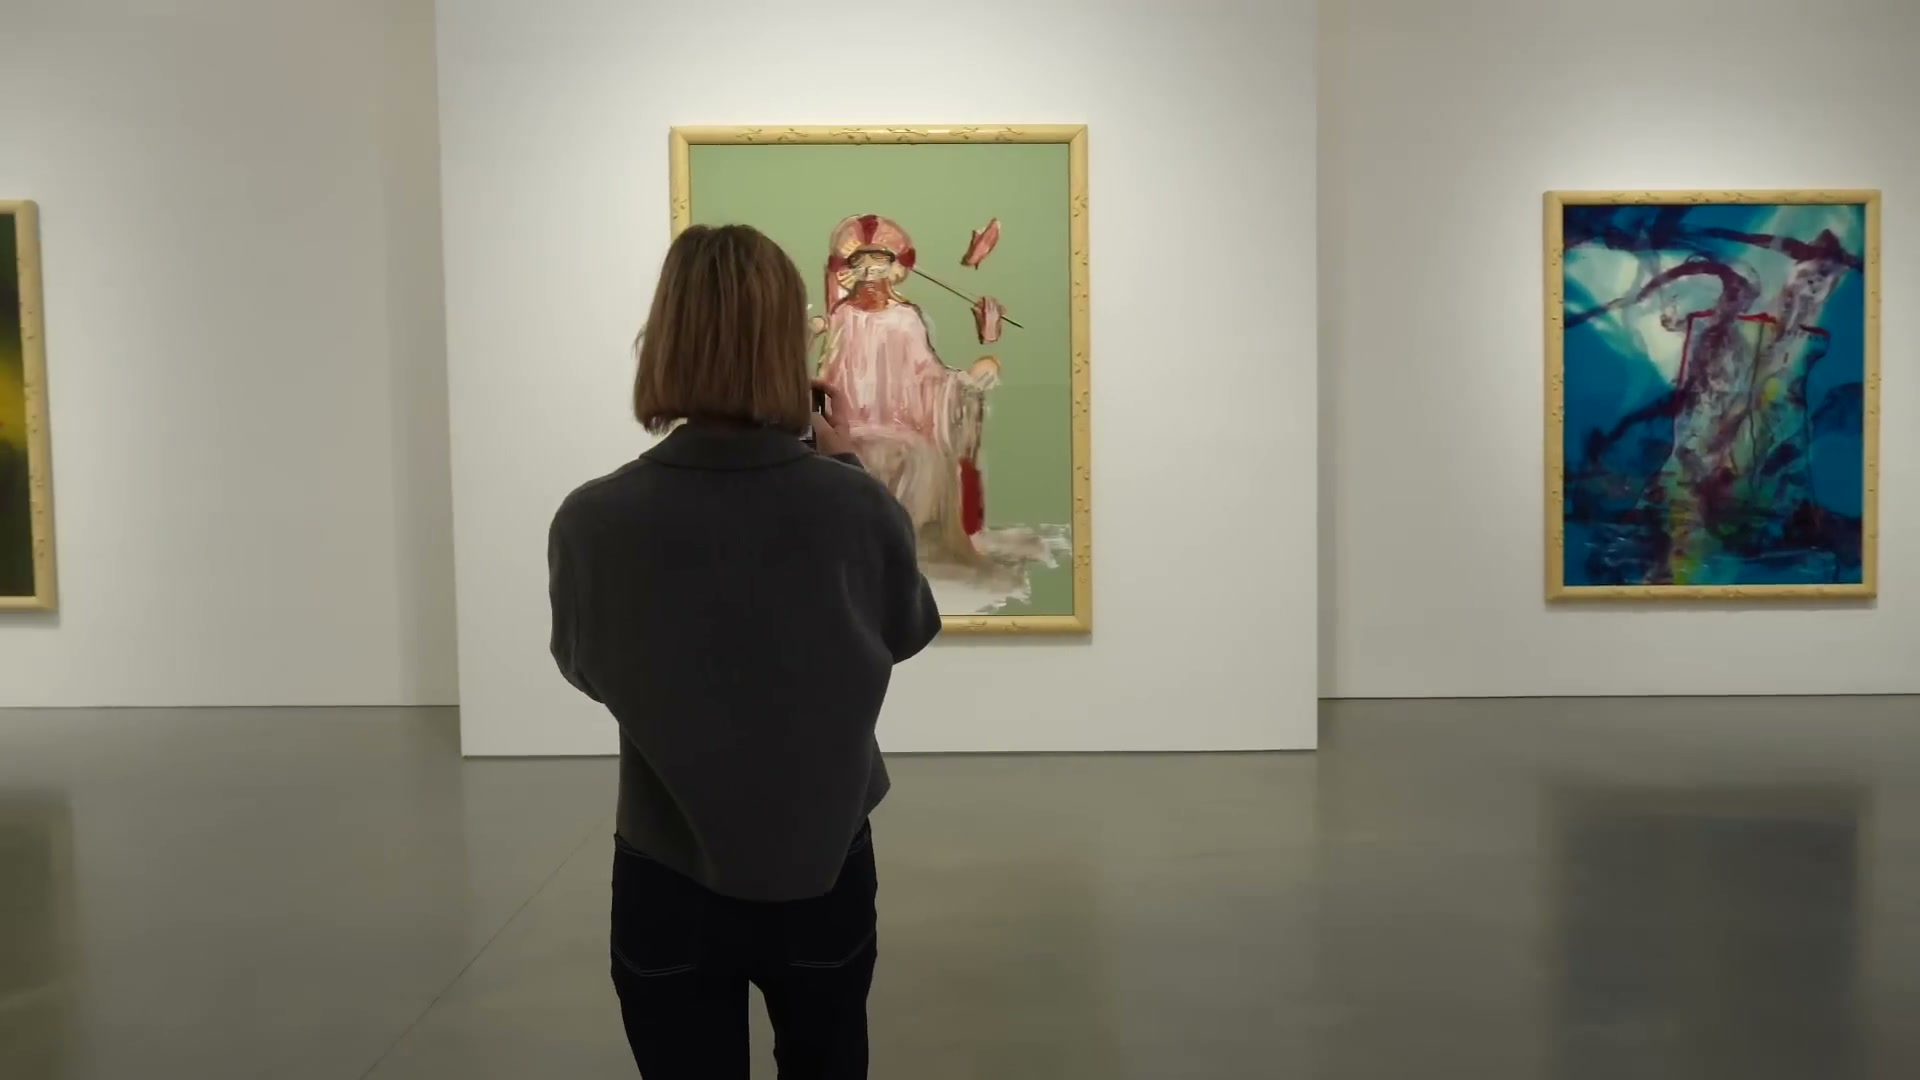
\includegraphics[width=0.97\linewidth]{src_frame.jpg}
\end{tikzfigure}
}

\block{From One Video, Four Products}{
Vitrine is a \emph{reconstruct-then-decompose} system. From one walkthrough it
delivers, in a single pass:
\vspace{2mm}

\begin{itemize}\setlength{\itemsep}{2.5mm}
\item a photoreal \textbf{Gaussian-splat field} of the whole space, the
      high-fidelity record;
\item a set of \textbf{named, individually-addressable objects}, each isolated
      from the field and placed at its measured pose;
\item a textured \textbf{polygonal environment} and per-object meshes, the
      games-engine-ready geometry; and
\item a single \textbf{USD scene graph} binding them together with
      source-video provenance, importable straight into Unreal.
\end{itemize}
\vspace{3mm}
The work \textbf{pairs with, and never forks}, the upstream \textbf{LichtFeld
Studio} reconstruction engine. Vitrine is the agentic orchestration,
segmentation, decomposition and assembly layer on top of it.
}

\block{Eight-Stage Agentic Pipeline}{
A swarm of specialist agents drives the full path from pixels to scene graph;
every stage is manifest-configured, checkpointed and independently recoverable.
\vspace{3mm}

\centering
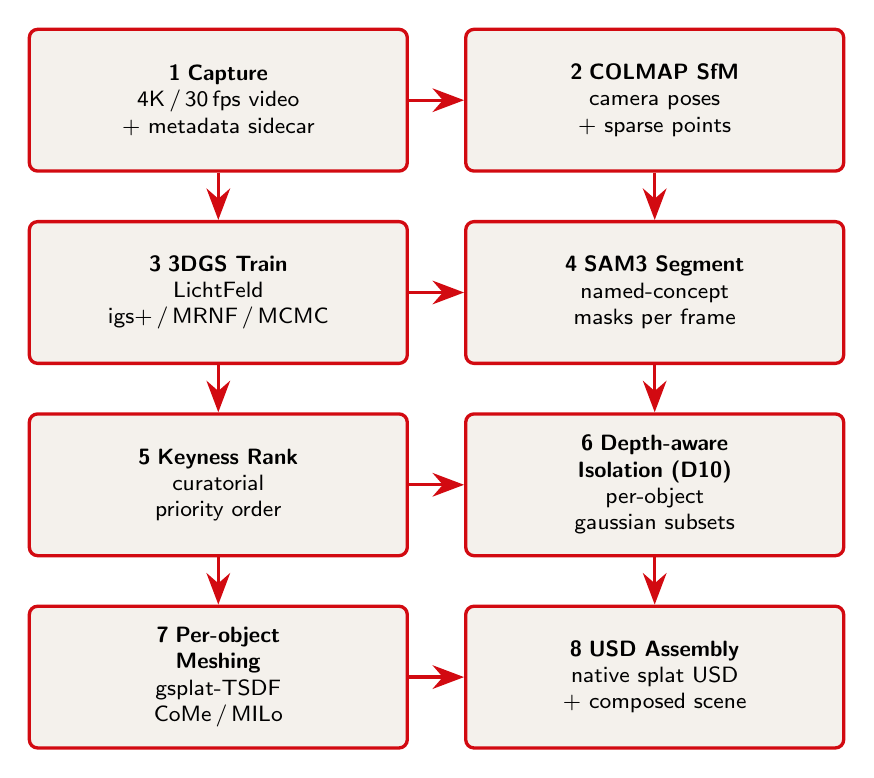
\begin{tikzpicture}[
  font=\footnotesize,
  node distance=6mm and 7mm,
  stg/.style={rectangle, rounded corners=3pt, draw=salfordred, very thick,
              fill=panelgrey, text width=44mm, align=center, minimum height=18mm,
              inner sep=2mm},
  ar/.style={-{Stealth[length=4mm]}, very thick, salfordred}]
\node[stg] (a) {\textbf{1\;Capture}\\4K\,/\,30\,fps video\\+ metadata sidecar};
\node[stg, right=of a] (b) {\textbf{2\;COLMAP SfM}\\camera poses\\+ sparse points};
\node[stg, below=of a] (c) {\textbf{3\;3DGS Train}\\LichtFeld\\igs+\,/\,MRNF\,/\,MCMC};
\node[stg, right=of c] (d) {\textbf{4\;SAM3 Segment}\\named-concept\\masks per frame};
\node[stg, below=of c] (e) {\textbf{5\;Keyness Rank}\\curatorial\\priority order};
\node[stg, right=of e] (f) {\textbf{6\;Depth-aware\\Isolation (D10)}\\per-object\\gaussian subsets};
\node[stg, below=of e] (g) {\textbf{7\;Per-object\\Meshing}\\gsplat-TSDF\\CoMe\,/\,MILo};
\node[stg, right=of g] (h) {\textbf{8\;USD Assembly}\\native splat USD\\+ composed scene};
\draw[ar] (a)--(b); \draw[ar] (a)--(c); \draw[ar] (b.south) to[out=-90,in=90] (d.north);
\draw[ar] (c)--(d); \draw[ar] (c)--(e); \draw[ar] (d.south) to[out=-90,in=90] (f.north);
\draw[ar] (e)--(f); \draw[ar] (e)--(g); \draw[ar] (f.south) to[out=-90,in=90] (h.north);
\draw[ar] (g)--(h);
\end{tikzpicture}
\vspace{2mm}

\small Two agents, cleanly separated: an \textbf{in-container orchestrator} that
decides what to run over the LichtFeld tool surface, and a \textbf{multimodal
vision agent} it calls for artefact judgement. No hidden state machine: explicit
tool-calls over a manifest.
}

\block{Photoreal Radiance Field}{
Stage~3 trains a 3D Gaussian-Splatting field with LichtFeld's
\texttt{igs+} strategy, giving real-time novel-view synthesis at capture
resolution.
\vspace{3mm}

\begin{tikzfigure}[Novel views rendered from the trained 4\,M-gaussian field.]
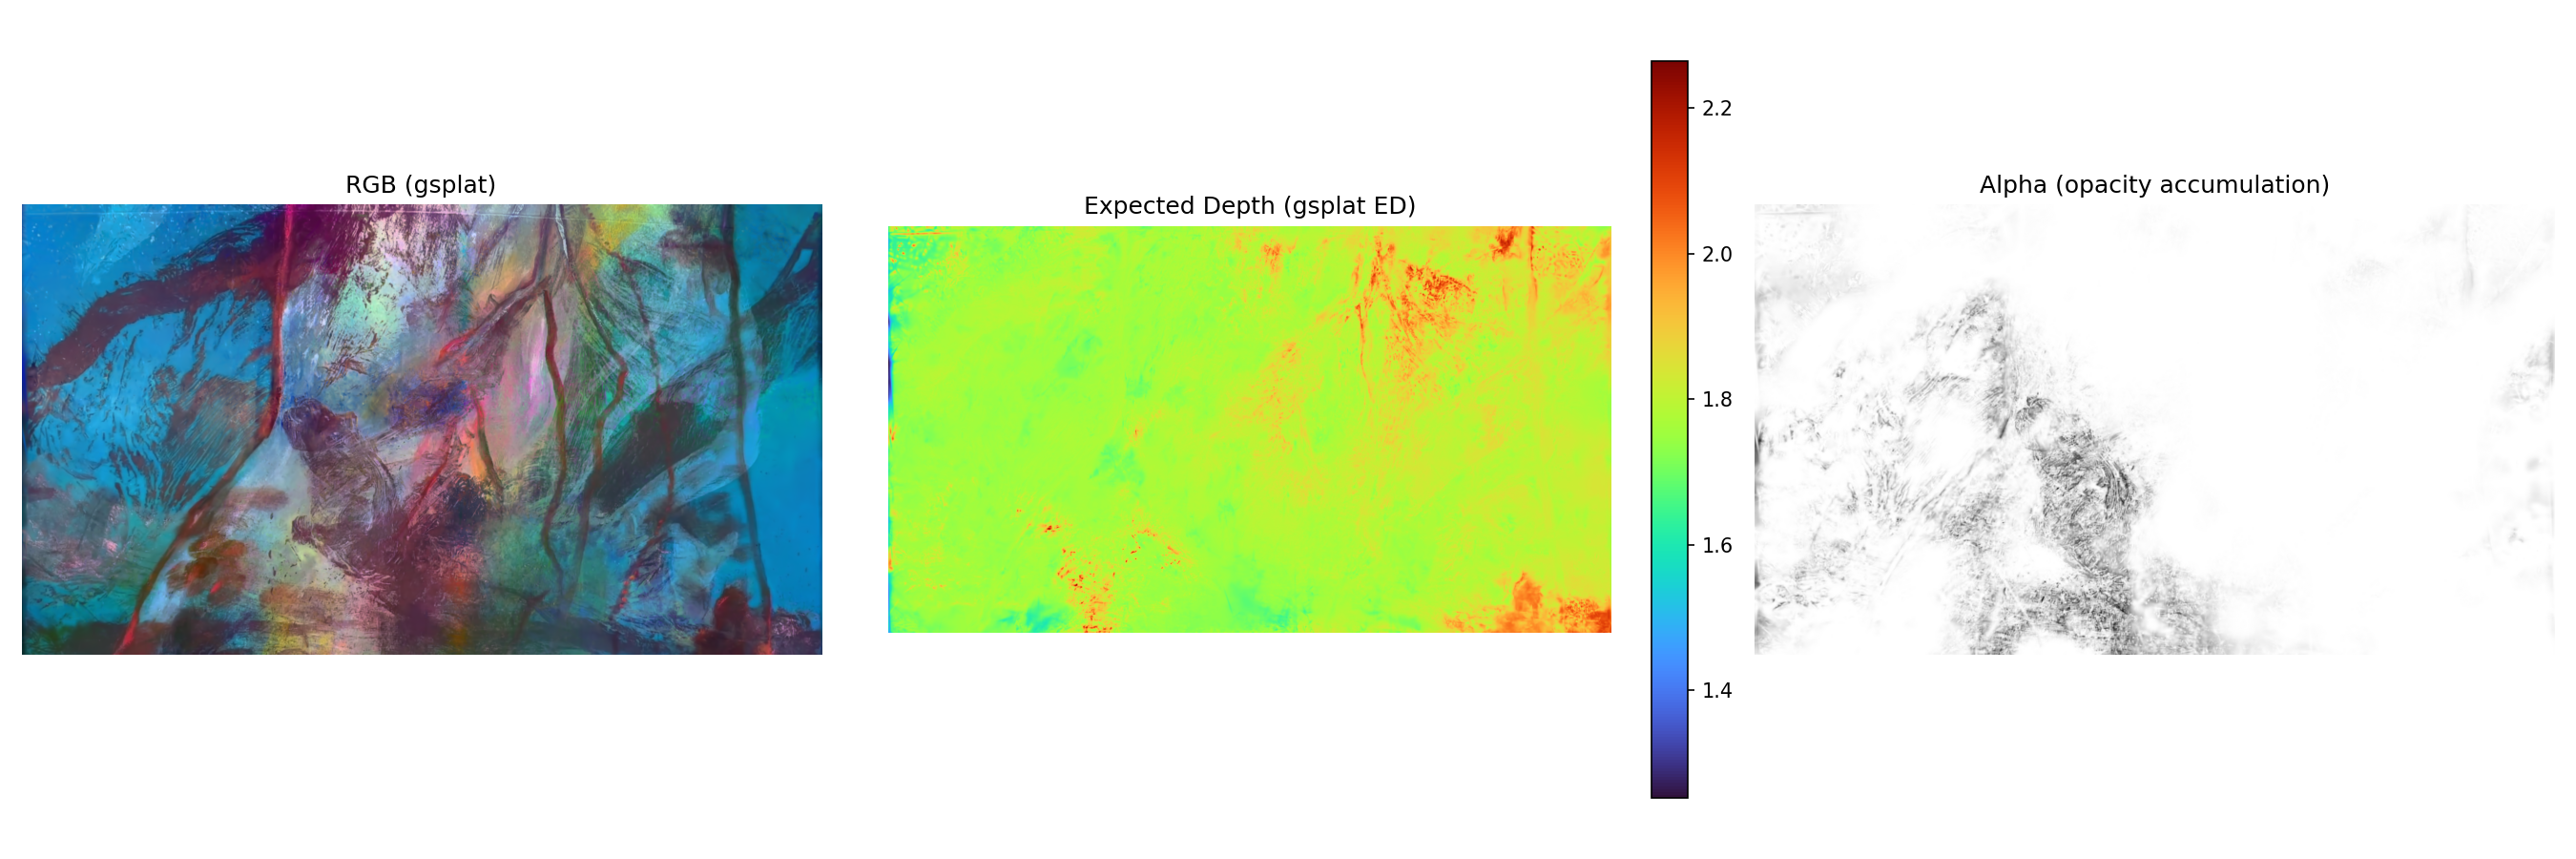
\includegraphics[width=0.98\linewidth]{splat_render.png}
\end{tikzfigure}
\vspace{3mm}

\begin{center}\large
\stat{4.0\,M}{gaussians}\;$\cdot$\;
\stat{80}{frames}\;$\cdot$\;
\stat{SH\,3}{harmonics}\\[3mm]
\stat{30\,000}{train iters}\;$\cdot$\;
\stat{901\,MB}{native USD}
\end{center}
}

% ======================================================================
% COLUMN 2
% ======================================================================
\column{0.34}

\block{Core Result: an Object-Resolved Scene}{
Vitrine's central contribution is moving from a \textbf{monolithic} radiance
field to a \textbf{structured, editable scene}. \textbf{SAM3} segments the
capture into named concepts; a new \textbf{depth-aware multi-view projection}
votes each gaussian inside or outside an object's masks across every registered
COLMAP camera, isolating each object into its own gaussian subset.
\vspace{3mm}

On the validated 80-frame scene this resolved \textbf{five named objects},
correctly ranked with the key items above the structural surfaces:
\vspace{2mm}

\renewcommand{\arraystretch}{1.28}
\begin{tabularx}{0.99\linewidth}{@{}lXr@{}}
\toprule
\textbf{Object} & \textbf{Role} & \textbf{Gaussians} \\
\midrule
\rowcolor{panelgrey}\textbf{Sculptures} & key item & 1{,}080{,}171 \\
\textbf{Furniture} & key item & 452{,}401 \\
\rowcolor{panelgrey}Floor & structure & 964{,}074 \\
Walls & structure & 357{,}276 \\
\rowcolor{panelgrey}Ceiling & structure & 11{,}012 \\
\bottomrule
\end{tabularx}
\vspace{2mm}

\small Keyness $=$ curatorial priority $\times$ gaussian count, so
\textbf{sculptures} and \textbf{furniture} rank above the floor despite the
floor's larger raw count.
}

\block{Hierarchical USD Scene Graph}{
Each isolated object becomes a USD prim under a single scene graph, carrying a
\textbf{Gaussian\,$|$\,Mesh variant set} and \texttt{v2g:*} provenance metadata
back to the source video.
\vspace{3mm}

\centering
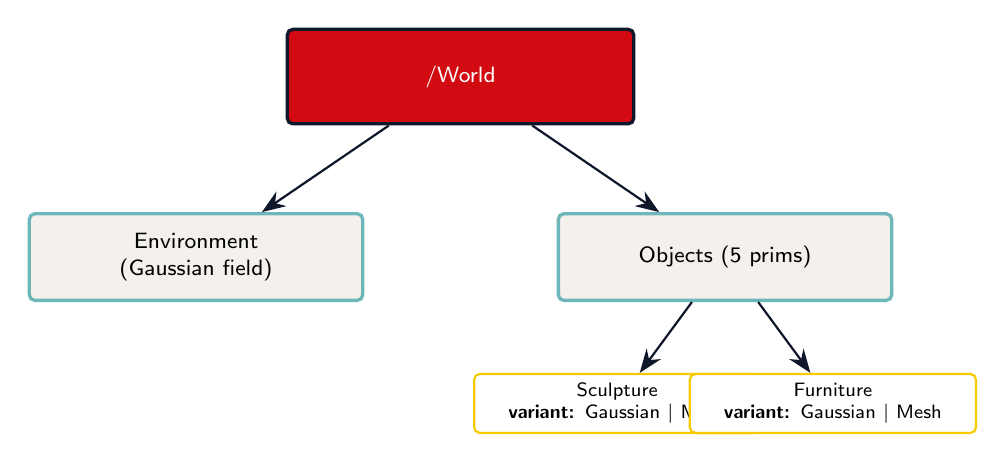
\begin{tikzpicture}[font=\footnotesize,
  rt/.style={rectangle, rounded corners=2pt, draw=salfordnavy, very thick,
             fill=salfordred, text=white, align=center, minimum width=44mm, minimum height=12mm},
  pr/.style={rectangle, rounded corners=2pt, draw=salfordteal, very thick, fill=panelgrey,
             align=center, text width=40mm, minimum height=11mm},
  vs/.style={rectangle, rounded corners=2pt, draw=salfordgold, thick, fill=white,
             align=center, text width=34mm, font=\scriptsize},
  ed/.style={-{Stealth[length=3mm]}, thick, salfordnavy}]
\node[rt] (w) {/World};
\node[pr, below left=11mm and -10mm of w] (env) {Environment\\(Gaussian field)};
\node[pr, below right=11mm and -10mm of w] (obj) {Objects (5 prims)};
\draw[ed] (w)--(env); \draw[ed] (w)--(obj);
\node[vs, below left=9mm and -26mm of obj] (v1) {Sculpture\\\textbf{variant:} Gaussian $|$ Mesh};
\node[vs, below right=9mm and -26mm of obj] (v2) {Furniture\\\textbf{variant:} Gaussian $|$ Mesh};
\draw[ed] (obj)--(v1); \draw[ed] (obj)--(v2);
\end{tikzpicture}
\vspace{3mm}

Two USD products ship together: a \textbf{native LichtFeld splat USD} (headless
CLI \texttt{convert}, 901\,MB) and a \textbf{composed, textured scene} assembled
in Blender with preview renders. A viewer can swap any object between its splat
appearance and a watertight polygonal twin without re-authoring the scene.
\vspace{3mm}

\begin{tikzfigure}[Composed multi-object scene: isolated objects re-emplaced at surveyed pose.]

\includegraphics[width=0.98\linewidth]{multi_object_composed.jpg}
\end{tikzfigure}
}

\block{Per-Object 360\textdegree{} Recovery}{
Objects seen from only one side are completed by a generative sub-pipeline, then
re-emplaced at their surveyed pose as separate, inference-reconstructed objects
inside the scene.
\vspace{3mm}

\centering
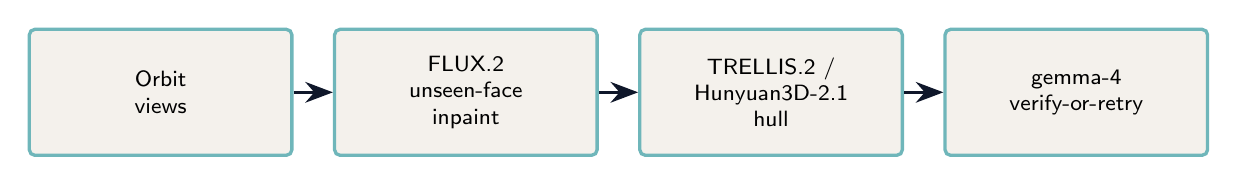
\begin{tikzpicture}[font=\footnotesize, node distance=5mm,
  s/.style={rectangle, rounded corners=2pt, draw=salfordteal, very thick, fill=panelgrey,
            text width=31mm, align=center, minimum height=16mm},
  a/.style={-{Stealth[length=3.5mm]}, very thick, salfordnavy}]
\node[s] (o1) {Orbit\\views};
\node[s, right=of o1] (o2) {FLUX.2\\unseen-face\\inpaint};
\node[s, right=of o2] (o3) {TRELLIS.2 /\\Hunyuan3D-2.1\\hull};
\node[s, right=of o3] (o4) {gemma-4\\verify-or-retry};
\draw[a] (o1)--(o2); \draw[a] (o2)--(o3); \draw[a] (o3)--(o4);
\end{tikzpicture}
\vspace{2mm}

\small A local \textbf{gemma-4} vision agent judges each recovered object and
loops back on failure. Output is a \textbf{textured, watertight PBR mesh}
emplaced at its measured pose.
}

% ======================================================================
% COLUMN 3
% ======================================================================
\column{0.32}

\block{Validated End-to-End, June 2026}{
A single walkthrough now travels the \textbf{whole path} on real data:
training $\rightarrow$ SAM3 segmentation $\rightarrow$ depth-aware isolation
$\rightarrow$ per-object meshing $\rightarrow$ dual-USD assembly.
\vspace{2mm}

\renewcommand{\arraystretch}{1.25}
\begin{tabularx}{0.99\linewidth}{@{}Xr@{}}
\toprule
\textbf{Stage} & \textbf{Result} \\
\midrule
LichtFeld 3DGS training & \stag{okgreen}{4.0\,M splat} \\
SAM3 concept segmentation & \stag{okgreen}{5 objects} \\
Depth-aware isolation (D10) & \stag{okgreen}{5 subsets} \\
Keyness ranking (FR-9) & \stag{okgreen}{ordered} \\
Per-object meshing & \stag{okgreen}{5 meshes} \\
Native USD export & \stag{okgreen}{901\,MB} \\
Composed textured USD & \stag{okgreen}{scene.usda} \\
Lifecycle + control suites & \stag{okgreen}{31/31} \\
\bottomrule
\end{tabularx}
\vspace{3mm}

\small Running the pipeline surfaced and fixed \textbf{eight concrete defects}:
the SAM\,3.1 \texttt{addmm\_act} bf16 regression, the gsplat SH-degree loader,
Hunyuan3D kwargs, LichtFeld CUDA-13 runtime libs, the D10 projection, the native
USD path, and two Blender~5.0 export bugs. Every one surfaced by \emph{running}
the pipeline, not by reading it.
}

\block{State-of-the-Art Model Stack}{
The pilot tracks 2026 frontier models, staged and version-pinned on the host:
\vspace{2mm}

\renewcommand{\arraystretch}{1.18}
\footnotesize
\begin{tabularx}{0.99\linewidth}{@{}lX@{}}
\toprule
\textbf{Role} & \textbf{Model} \\
\midrule
Splat training & LichtFeld Studio (igs+) \\
Segmentation & SAM3 concept masks \\
Matching & ALIKED + LightGlue \\
Object hulls & TRELLIS.2 · Hunyuan3D-2.1 \\
Face recovery & FLUX.2-dev \\
Vision judge & gemma-4-26B-A4B \\
Mesh backends & gsplat-TSDF · CoMe · MILo \\
\bottomrule
\end{tabularx}
\vspace{3mm}

\begin{tikzfigure}[Per-object mesh reconstruction of the captured interior.]
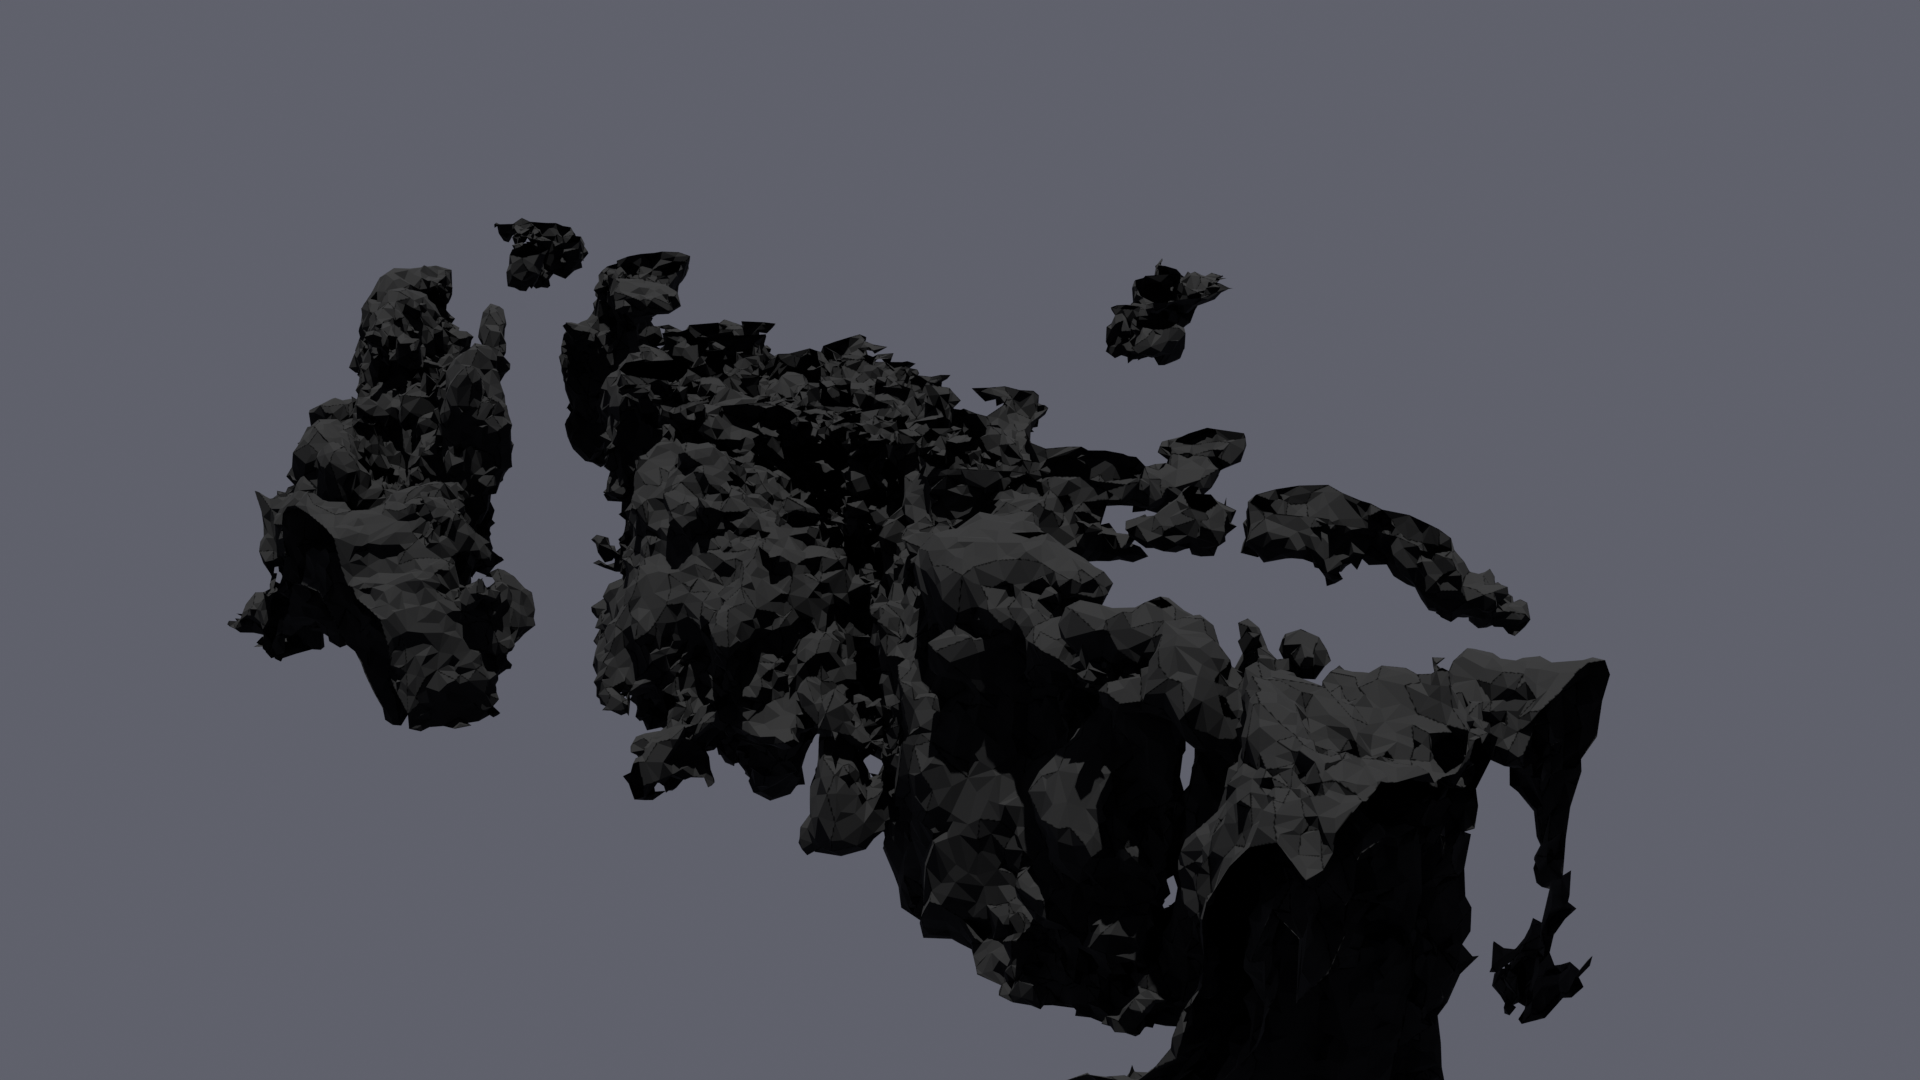
\includegraphics[width=0.99\linewidth]{gsplat_mesh.png}
\end{tikzfigure}
}

\block{System Architecture}{
A manifest-driven control plane runs a heterogeneous GPU toolchain across
\textbf{three coordinated containers} on a \texttt{v2g-net} service mesh:
\vspace{2mm}

\begin{itemize}\setlength{\itemsep}{1.8mm}
\item \textbf{Single \texttt{exhibit.toml} manifest}: one human-authored input;
      \texttt{env:} secret indirection; pre-snapshot stripping.
\item \textbf{Serial model lifecycle}: VRAM-bounded soft/hard unload; peak
      $=\max$(stage), not the sum.
\item \textbf{Agent-controlled ComfyUI} plus a SOTA model registry with a host
      ``idiot-check'' wired into preflight.
\item \textbf{Rust/Axum web onboarding}: a six-step wizard that round-trips the
      manifest with verified secret containment.
\end{itemize}
\vspace{2mm}
\small Built on \textbf{LichtFeld Studio} with native USD I/O and an MCP control
server. Reference host: dual \textbf{RTX~6000 Ada} class GPUs.
\vspace{3mm}

\begin{tikzfigure}[Schema-driven web onboarding wizard.]
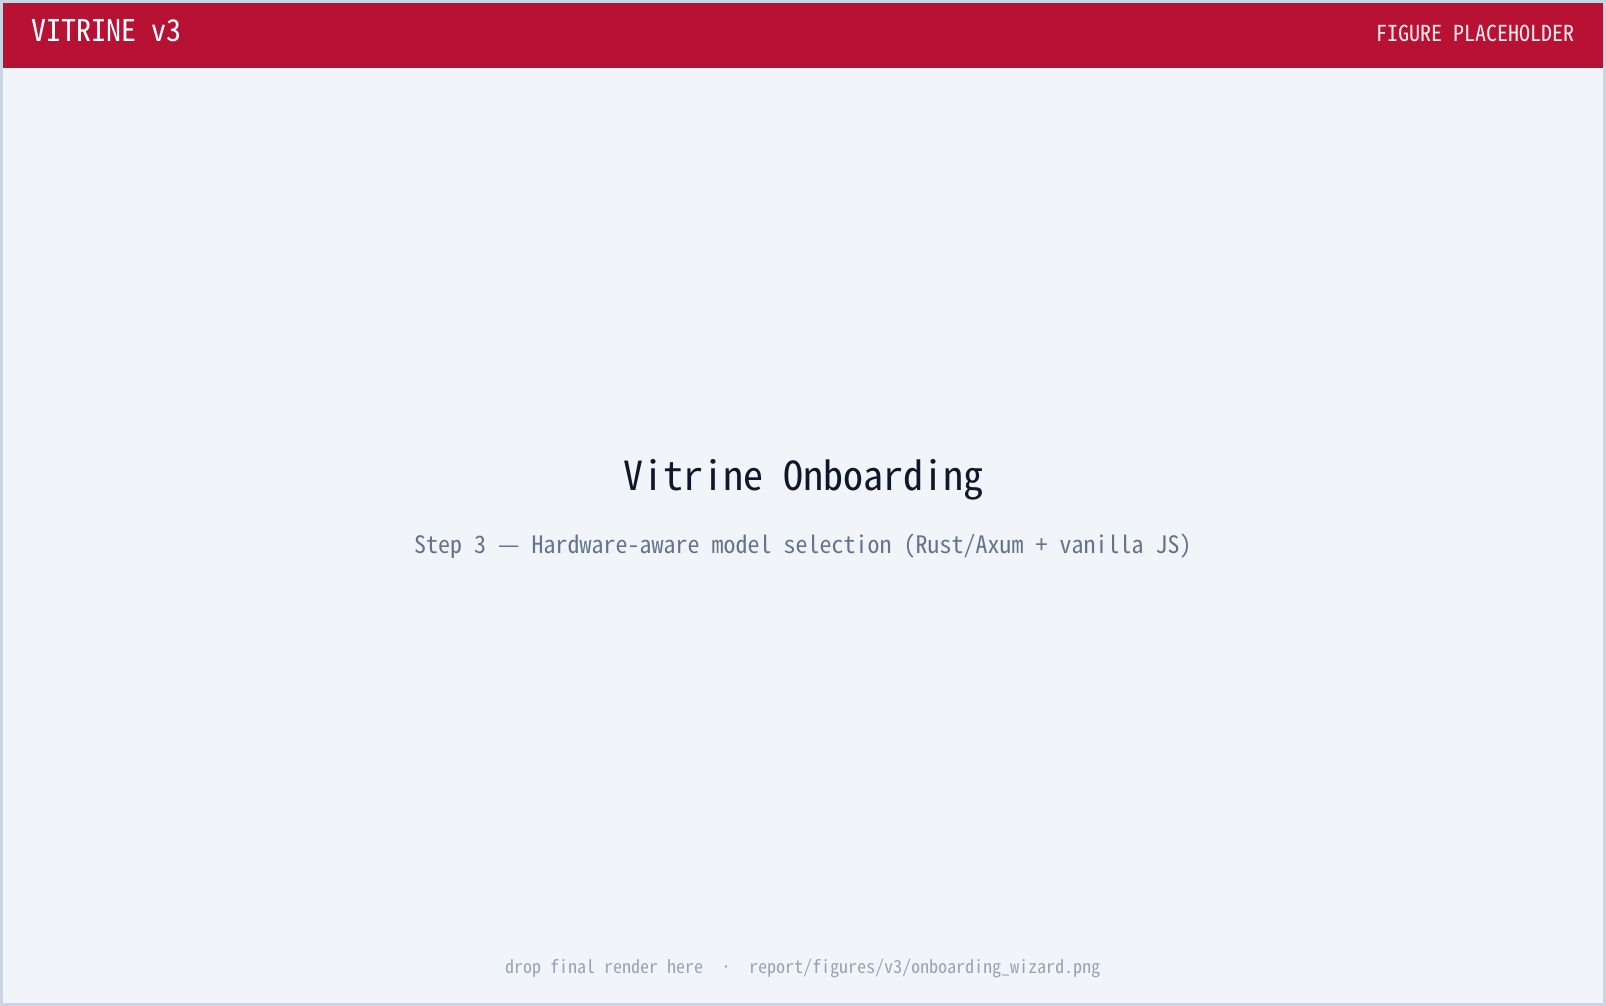
\includegraphics[width=0.99\linewidth]{onboarding_wizard.png}
\end{tikzfigure}
}

\block{Impact \& Roadmap}{
\textbf{For Salford:} a proof-of-principle toolset and business case for a
games-engine preservation space, plus cross-disciplinary CPD and knowledge
exchange for academic and technical staff, with IP negotiated for civic value
(open-source and Creative Commons).
\vspace{2mm}

\begin{enumerate}\setlength{\itemsep}{1.5mm}
\item \textbf{Pilot}: gallery capture \& end-to-end validation \emph{(done)}
\item \textbf{Quality \& SOTA hulls}: denser sampling, single-image hulls
\item \textbf{Fresh capture}: Drive\,$\rightarrow$\,ingest\,$\rightarrow$\,scene
\item \textbf{Scale}: multi-room collections in the MetaCampus
\end{enumerate}
\vspace{2mm}
\small Aligned to \textbf{EU Horizon Europe 2027} (Cluster~2,
HERITAGE-08: safeguarding intangible cultural heritage) with ARA, ICA, Rhizome
and Onassis ONX.
}

\note[targetoffsetx=0cm, targetoffsety=0cm, width=0.30\linewidth, connection=false, radius=0cm]{
\textbf{Programme:} University of Salford AI KE Community of Practice pilot \\
\textbf{Delivery partner:} DreamLab AI Consulting Ltd \;$\cdot$\; dreamlab-ai.com \\
\textbf{Engine:} LichtFeld Studio \;$\cdot$\; 3DGS \;$\cdot$\; SAM3 \;$\cdot$\; USD
}

\end{columns}

\end{document}
